\documentclass[aspectratio=169]{beamer}
\usepackage[utf8]{inputenc}
\usepackage{tikz} % for QR code overlay

% code snippets
\usepackage{minted}
\newmintedfile[dockercode]{dockerfile}{
  % bgcolor=mintedbackground,
  fontfamily=tt,
  linenos=true,
  numberblanklines=true,
  numbersep=5pt,
  gobble=0,
  frame=leftline,
  framerule=0.4pt,
  framesep=2mm,
  funcnamehighlighting=true,
  tabsize=4,
  obeytabs=false,
  mathescape=false
  samepage=false, %with this setting you can force the list to appear on the same page
  showspaces=false,
  showtabs =false,
  texcl=false,
}
\newminted[bashcode]{bash}{
  % bgcolor=mintedbackground,
  fontfamily=tt,
  linenos=true,
  numberblanklines=true,
  numbersep=5pt,
  gobble=0,
  frame=leftline,
  framerule=0.4pt,
  framesep=2mm,
  funcnamehighlighting=true,
  tabsize=4,
  obeytabs=false,
  mathescape=false
  samepage=false, %with this setting you can force the list to appear on the same page
  showspaces=false,
  showtabs =false,
  texcl=false,
}

% biblatex (requires biber; sudo pacman -S biber)
\usepackage[]{biblatex} % biblatex
\addbibresource{./src/bib/fhe.bib}
\addbibresource{./src/bib/dl.bib}
\addbibresource{./src/bib/misc.bib}

\usepackage{graphicx}
\graphicspath{ {./src/img/} }

\usetheme{Boadilla}
\usecolortheme{rose}
% \beamerdefaultoverlayspecification{<+->} % this will turn it into slides

\title{Augmented Agronomist}
\subtitle{Synthesis of Privacy-Preserving Deep Learning and Robotics to Assist Decision Support}
\author{George Onoufriou\\University of Lincoln}
\date{\today}

\begin{document}

\addtobeamertemplate{frametitle}{}{%
\begin{tikzpicture}[remember picture,overlay]
\node[anchor=north east,yshift=2pt] at (current page.north east) {
\includegraphics[height=1.5cm]{qrcode.png}};
\end{tikzpicture}}

  \frame{\titlepage}

% ----- ABOUT ME PAGE
  \begin{frame}
    \frametitle{About}
    \begin{columns}
      \begin{column}{0.5\textwidth}
        Myself:
        \begin{itemize}
          \item PhD Candidate Computer/ Data Science
          \item Privacy and Linux Enthusiast
        \end{itemize}
        Presentation:
        \begin{itemize}
          \item Slides are available via the QR code or link (QR available on every slide)
          \item Submit an issue in repository if seeing this later but still have questions
          \item Broad overview of yield prediction/ neural network techniques
        \end{itemize}
      \end{column}
      \begin{column}{0.5\textwidth}
        \begin{figure}[th!]
          \centering
          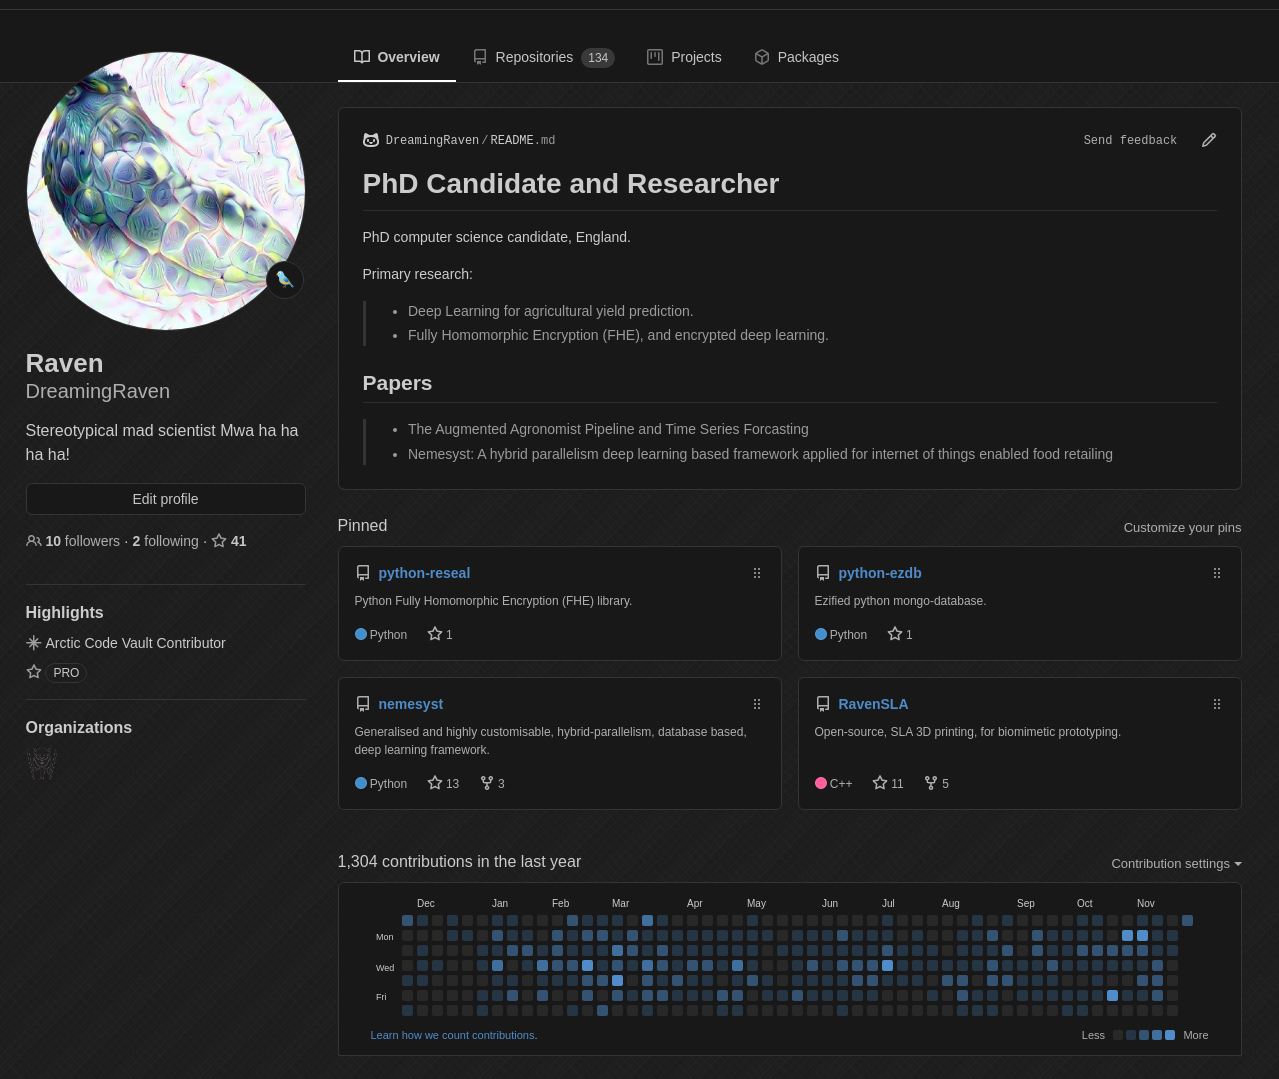
\includegraphics[width=0.8\textwidth]{gh.png}
          \caption{GitHub profile page where you can come to see my work and chat. \autocite{repository}}
          \label{fig:gh}
        \end{figure}
      \end{column}
    \end{columns}
  \end{frame}

% ----- PROBLEM PAGE
  \begin{frame}
    \frametitle{The Agricultural Problem}
    \begin{columns}
      \begin{column}{0.5\textwidth}
        Problem:
        \begin{itemize}
          \item How do you know how much produce any given farm will produce in $x$ weeks time
            \begin{itemize}
              \item 14\%
              \item 50\%
            \end{itemize}
          \item Either
            \begin{itemize}
              \item Have too much (storage, handling, disposal)
              \item Have too little (meeting agreements by importing, competition)
            \end{itemize}
        \end{itemize}
      \end{column}
      \begin{column}{0.5\textwidth}
        \begin{figure}[th!]
          \centering
          \includegraphics[width=0.6\textwidth]{waste.jpg}
          \caption{Waste from early on in the strawberry season starting to pile up. \autocite{repository}}
          \label{fig:gh}
        \end{figure}
      \end{column}
    \end{columns}
  \end{frame}

% ----- YIELD PROBLEM PAGE
  \begin{frame}
    \frametitle{Yield}
    \begin{columns}
      \begin{column}{0.3\textwidth}
        How do you account for:
        \begin{itemize}
          \item High variance between crops, crop locations, and varieties
          \item High variance in behavior of a single crop over a season
          \item High variance between growers
        \end{itemize}
      \end{column}
      \begin{column}{0.7\textwidth}
        \begin{figure}[th!]
          \centering
          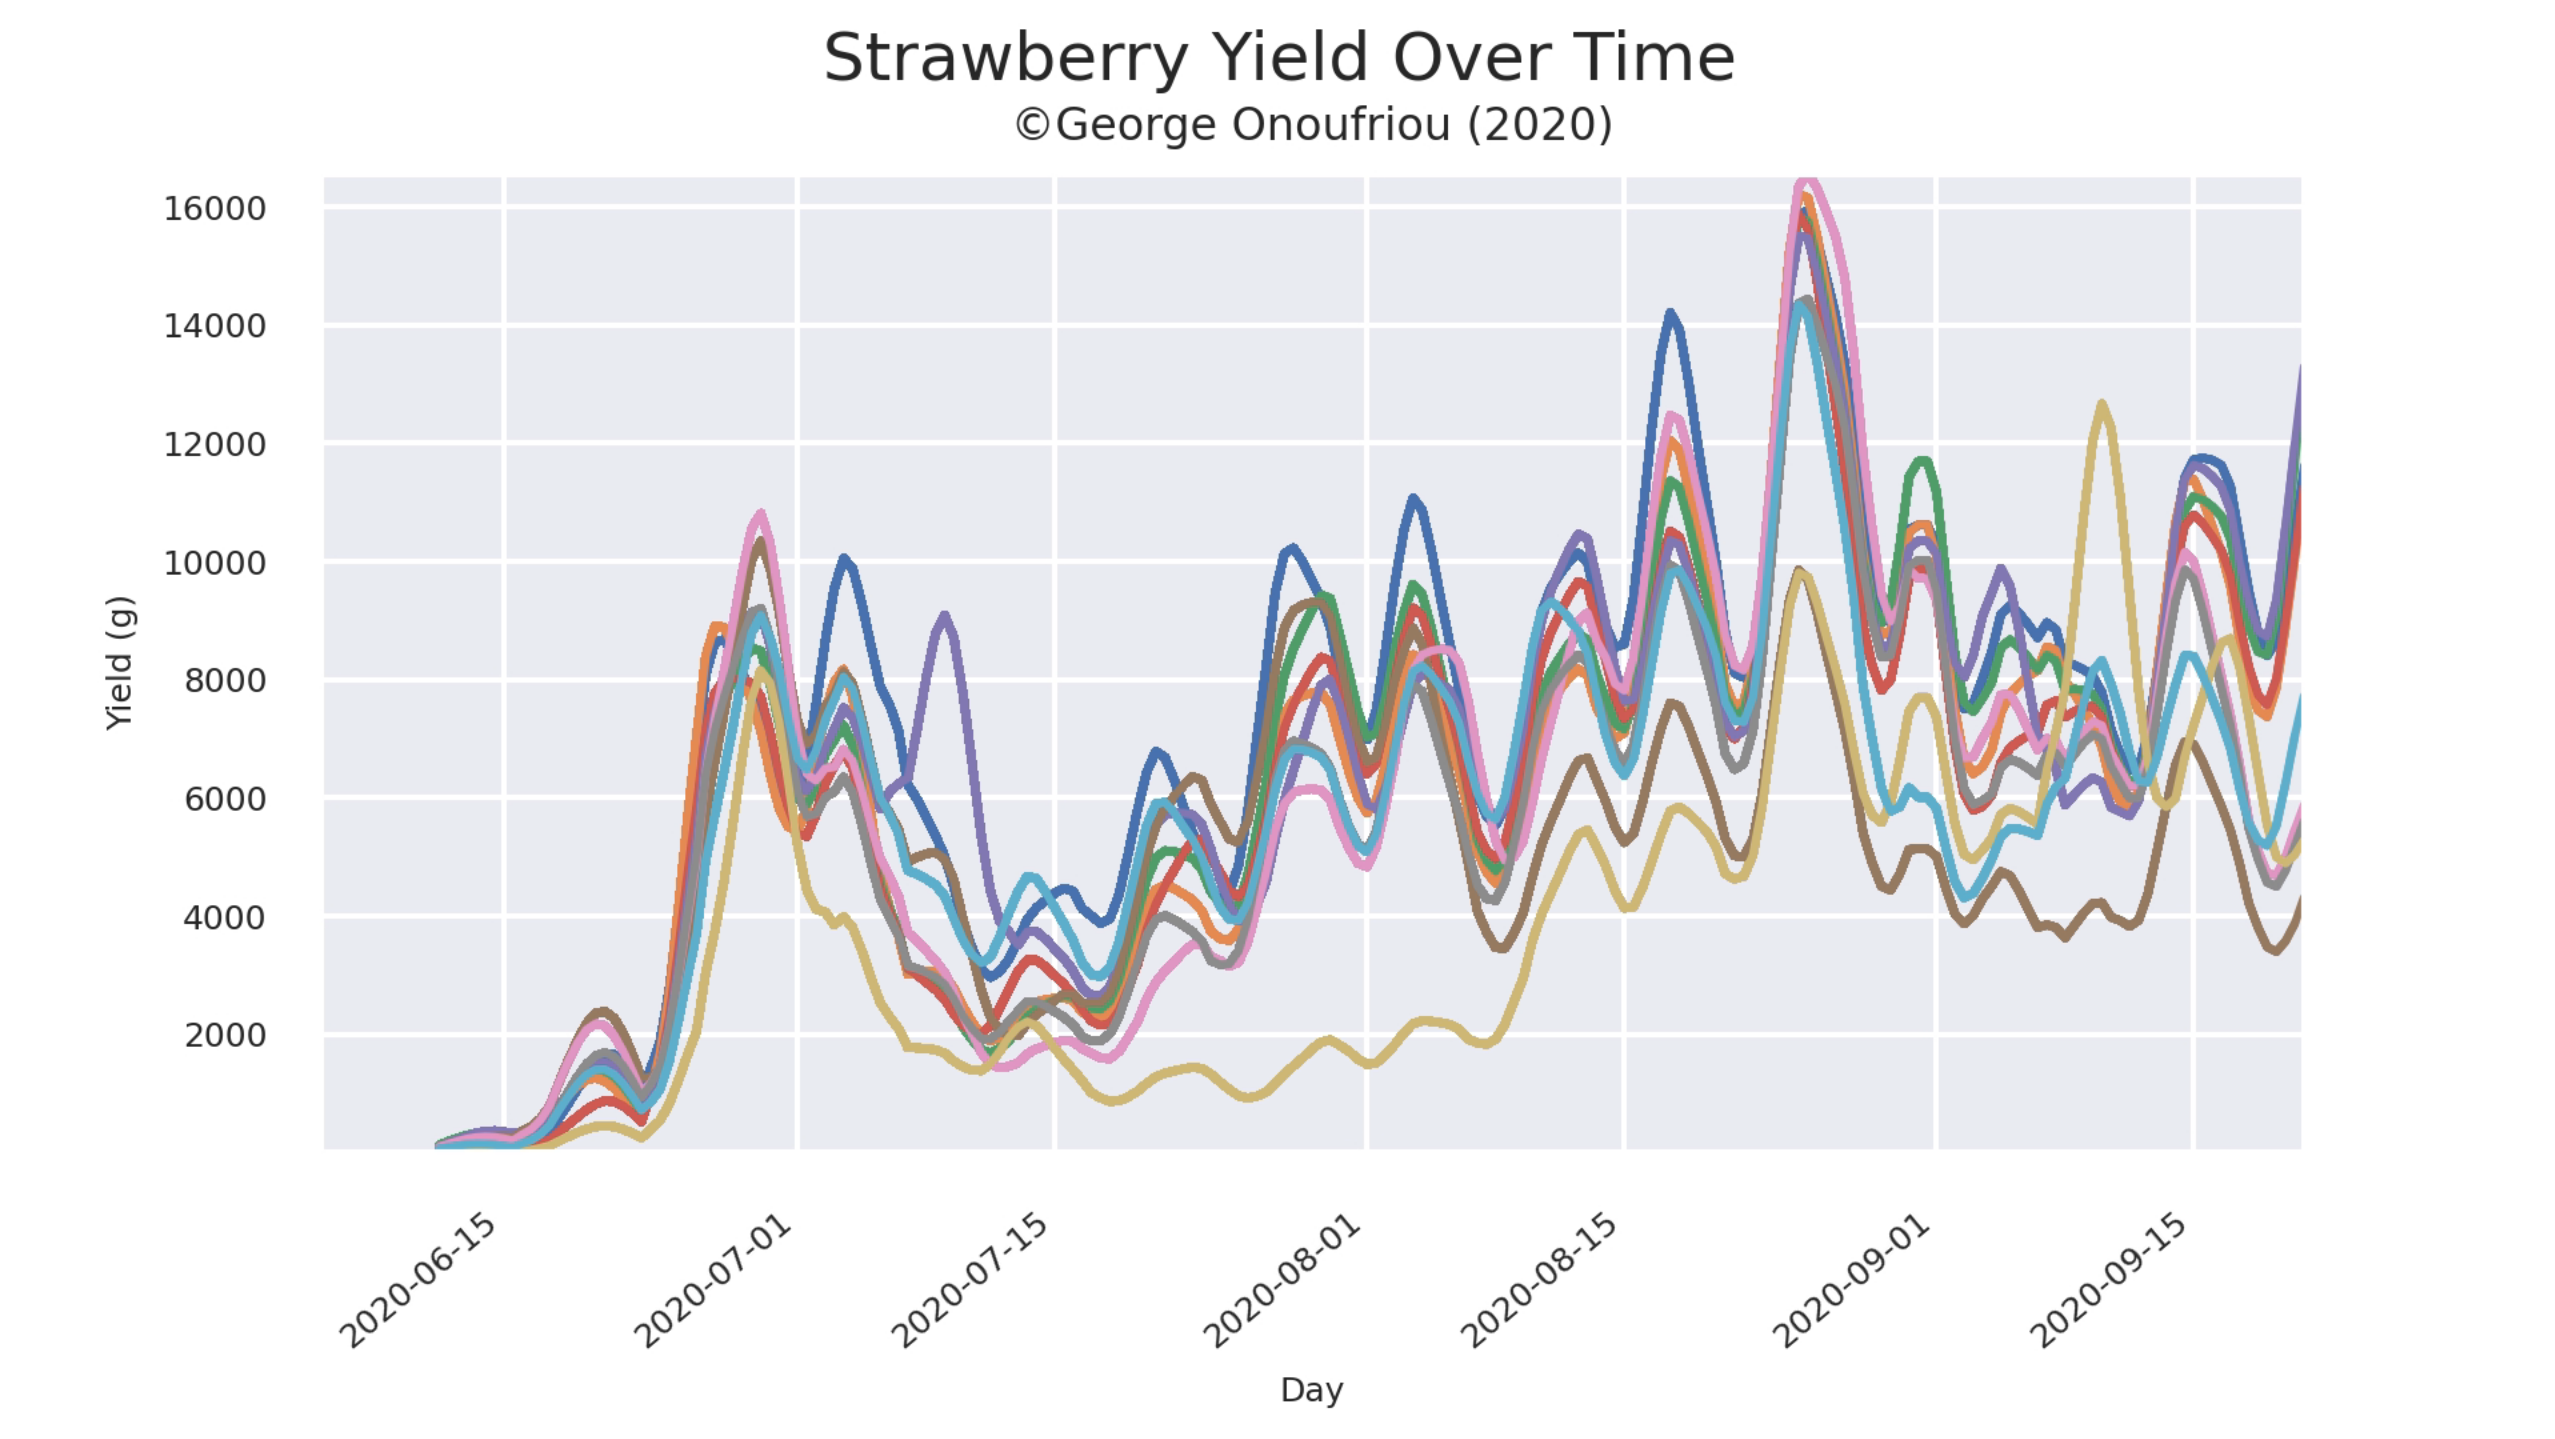
\includegraphics[width=1\textwidth]{yield.png}
          \caption{Yield over a portion of a season example. \autocite{repository}}
          \label{fig:yield}
        \end{figure}
      \end{column}
    \end{columns}
  \end{frame}

% ----- DATA PROBLEM PAGE
  \begin{frame}
    \frametitle{Data}
    \begin{columns}
      \begin{column}{0.5\textwidth}
        How can we use data to predict yield:
        \begin{itemize}
          \item Spacial; positions, images of plant and environment, movement, growth. (less common)
          \item Temporal; light, temperature, humidity, precipitation, irrigation, nutrition, wind-speed, etc. (common)
        \end{itemize}
        How readily available is this data:
        \begin{itemize}
          \item expensive equipment
          \item sensitivity to the data, e.g trade-secrets
          \item difficulty to obtaining and sharing
        \end{itemize}
      \end{column}
      \begin{column}{0.5\textwidth}
        \begin{figure}[th!]
          \centering
          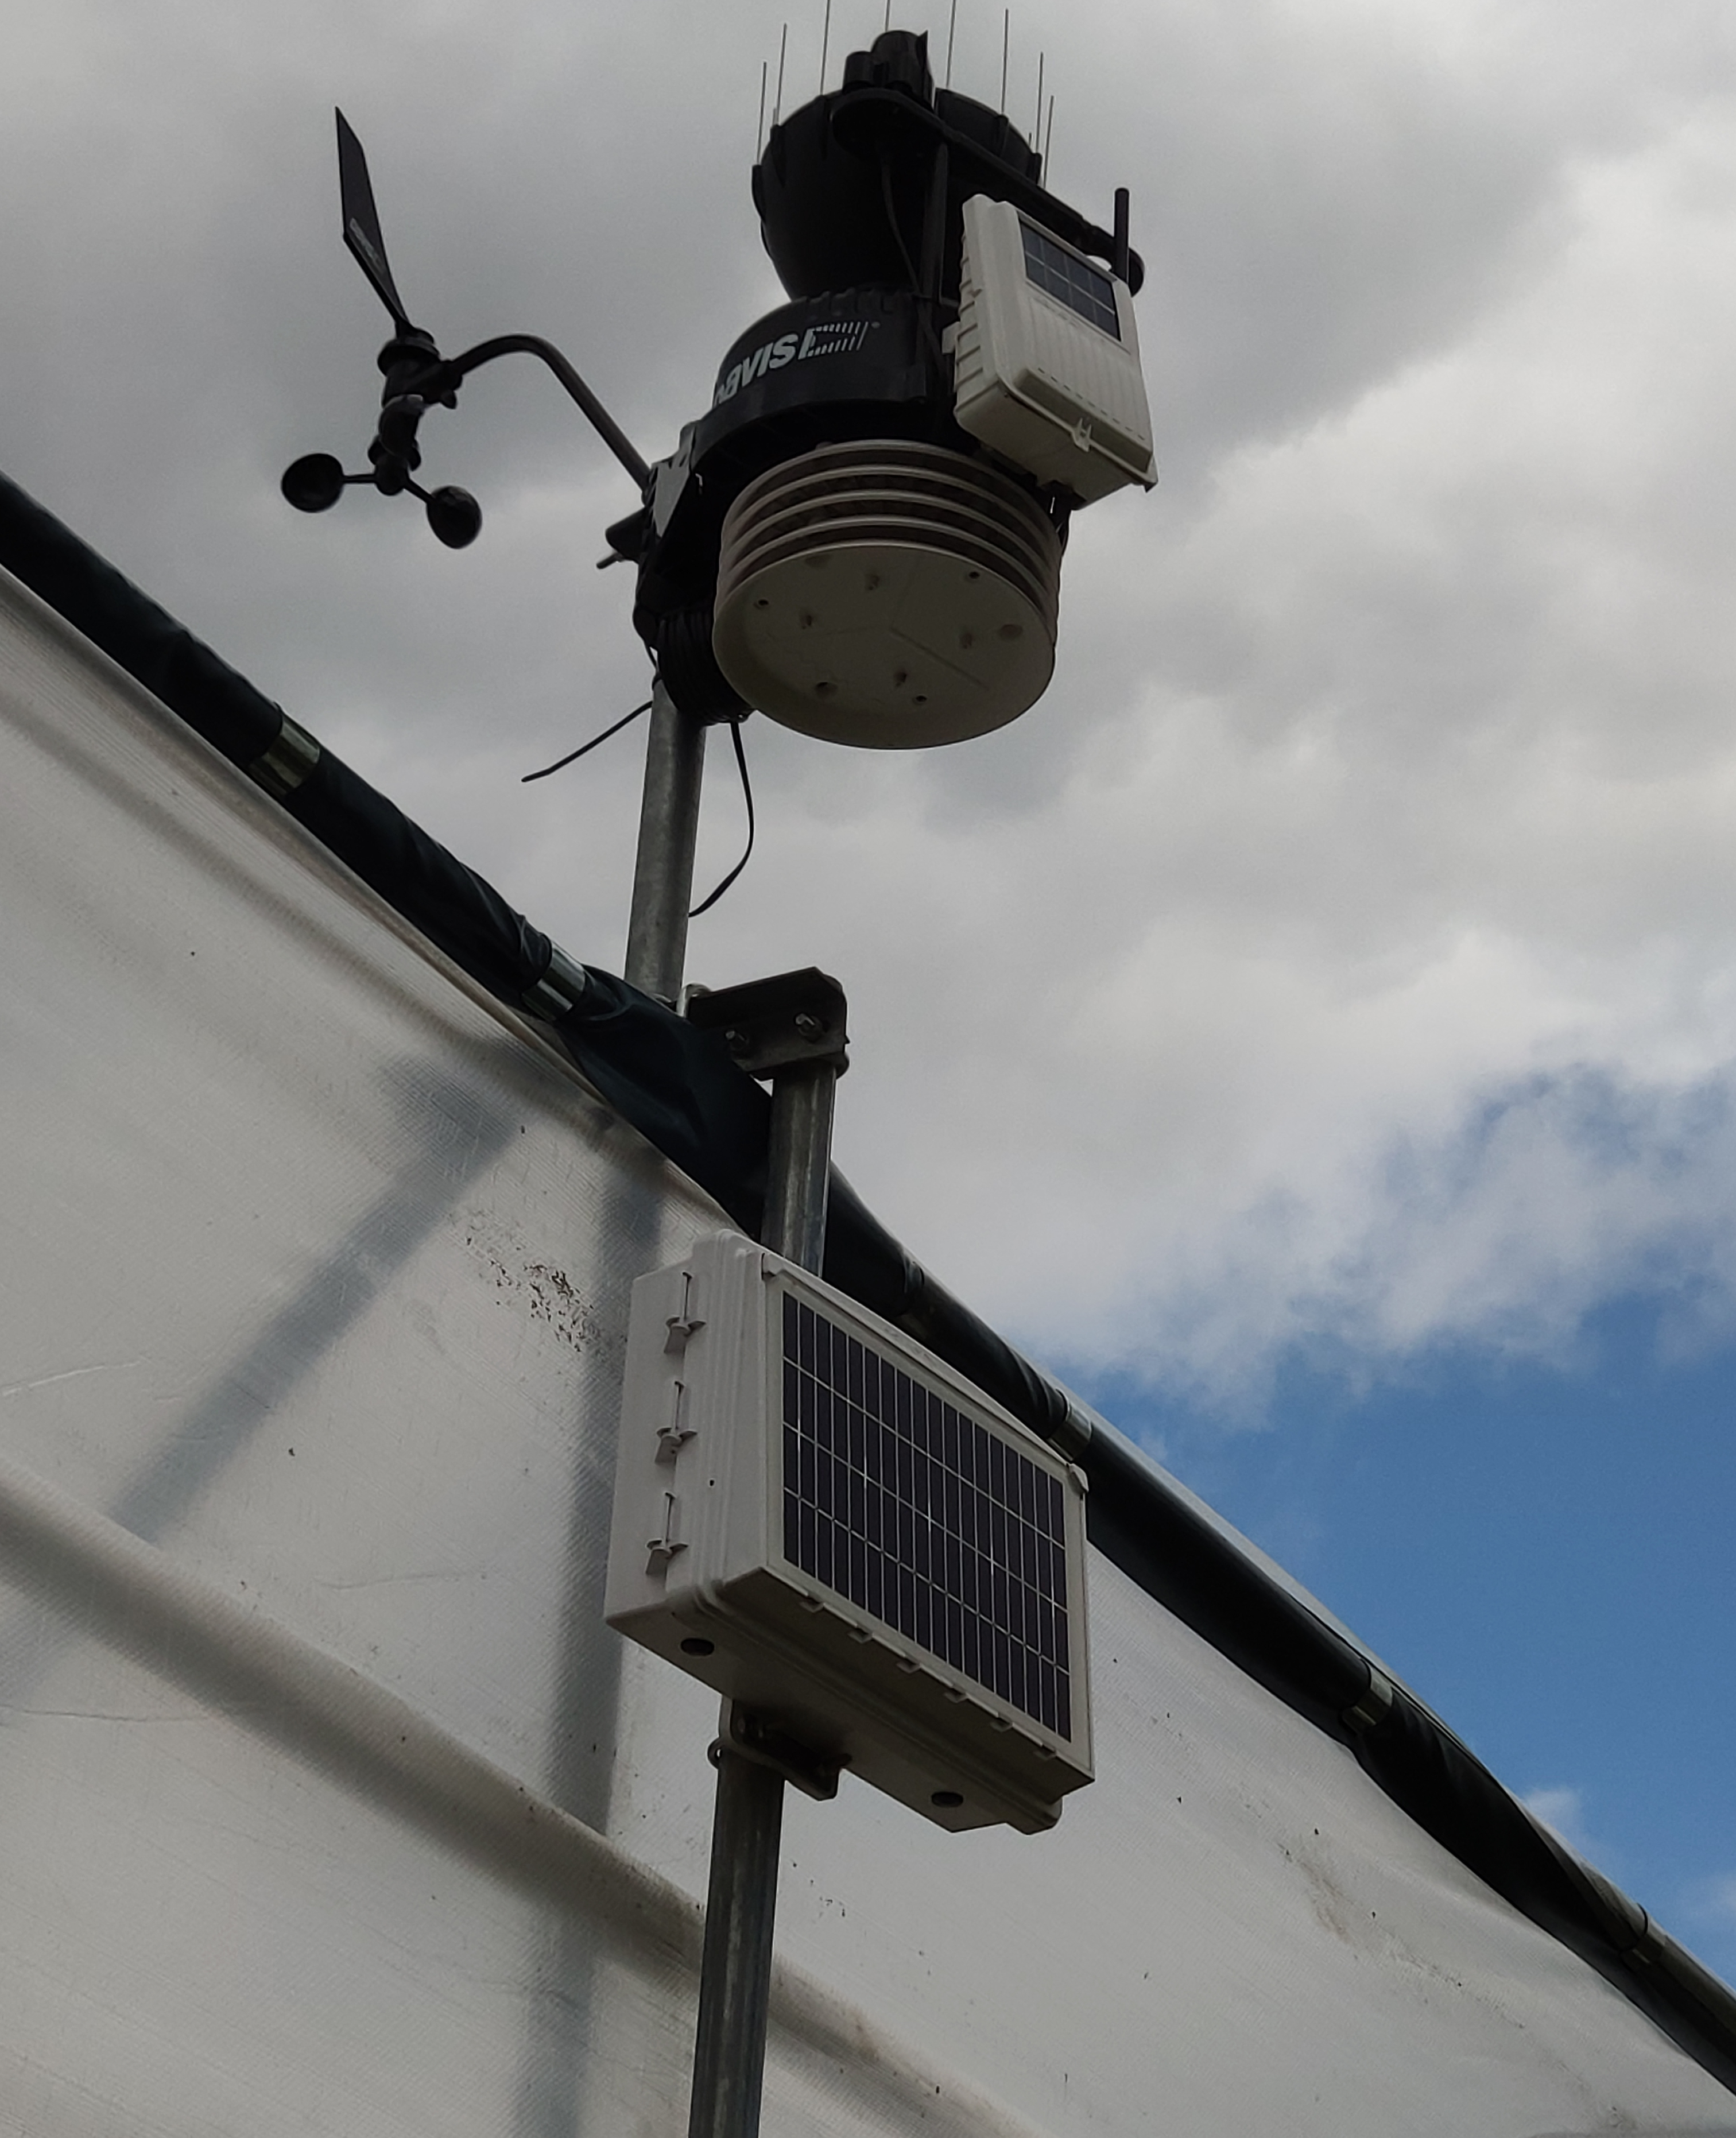
\includegraphics[width=0.55\textwidth]{weather.jpg}
          \caption{Weathervane collecting environmental data in regular intervals. \autocite{repository}}
          \label{fig:yield}
        \end{figure}
      \end{column}
    \end{columns}
  \end{frame}

% ----- MY WORK PAGE
  \begin{frame}
    \frametitle{My Work}
    \begin{columns}
      \begin{column}{0.5\textwidth}
        I work with:
        \begin{itemize}
          \item Deep Learning
          \item Fully Homomorphic Encryption \autocite{gentry2009fully}
        \end{itemize}
        Applied to:
        \begin{itemize}
          \item Agriculture; Predicting plant yield, in particular strawberries
        \end{itemize}
        Goals:
        \begin{itemize}
          \item Accurately predict yield
          \item Provide certainty in predictions for agronomist focus and re-prediction
          \item Privacy-preservation
        \end{itemize}
      \end{column}
      \begin{column}{0.5\textwidth}
        \begin{figure}[th!]
          \centering
          \includegraphics[angle=-90,origin=c,width=0.55\textwidth]{wasp.jpg}
          \caption{Strawberry tabletop with a wasp having some lunch. \autocite{repository}}
          \label{fig:wasp}
        \end{figure}
      \end{column}
    \end{columns}
  \end{frame}

% ----- DEEP LEARNING PAGE
  \begin{frame}
    \frametitle{Deep Learning + Fully Homomorphic Encryption}
    \begin{columns}
      \begin{column}{0.5\textwidth}
        Using:
        \begin{itemize}
          \item Deep learning/ neural networks
          \begin{itemize}
            \item Accurate predictions
            \item Timely manner
            \item Self assess certainty
            \item Adapt to various scenarios
          \end{itemize}
          \item Fully Homomorphic Encryption
          \begin{itemize}
            \item Process cyphertexts directly without the keys to them
            \item Quantum resistant mathematical problem (ring learning with errors)
            \item Process floating point numbers (CKKS \autocite{ckks})
          \end{itemize}
        \end{itemize}
      \end{column}
      \begin{column}{0.5\textwidth}
        \begin{figure}[th!]
          \centering
          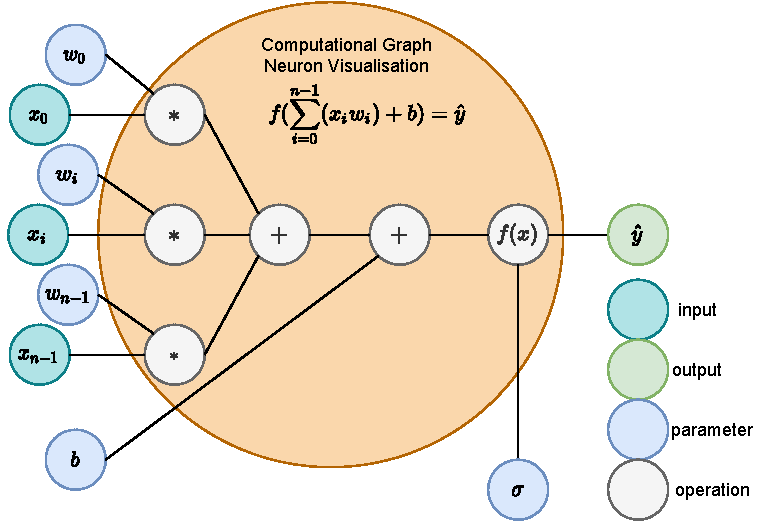
\includegraphics[width=0.8\textwidth]{neuron_computational_graph.pdf}
          \caption{Artificial Neural Network (ANN) neuron computational graphs. \autocite{repository}}
          \label{fig:ann_cg}
        \end{figure}
      \end{column}
    \end{columns}
  \end{frame}

% ----- RESULTS PAGE
  \begin{frame}
    \frametitle{Results}
    \begin{columns}
      \begin{column}{0.5\textwidth}

        \begin{table}[h]
        \begin{tabular}{lc}
          \hline
          Technique & MAE\\ \hline
          Recurrent Neural Networks       & 0.210     \\ % 14.2 / 67.52173913043478
          Long Short-Term Memory     & 0.381     \\ % 25.7 / 67.52
          Gated Recurrent Units       & 0.155     \\ \hline % 10.5 / 67.52
          \end{tabular}
          \label{tab:results}
        \end{table}
        Initial results trialing different sorts of neural networks for 2 week predictions.

        \begin{table}[h]
        \begin{tabular}{ll}
        Days Ahead & \begin{tabular}[c]{@{}l@{}}MAPE\end{tabular} \\ \hline
        7          & 8.001                                                                               \\
        14         & 14.669                                                                              \\
        21         & 22.326
        \end{tabular}
        \end{table}
        More recent results combining FHE + CNN + ANN as can be seen in fig \ref{fig:cnn_cg} adjacent.
      \end{column}
      \begin{column}{0.5\textwidth}
        \begin{figure}[th!]
          \centering
          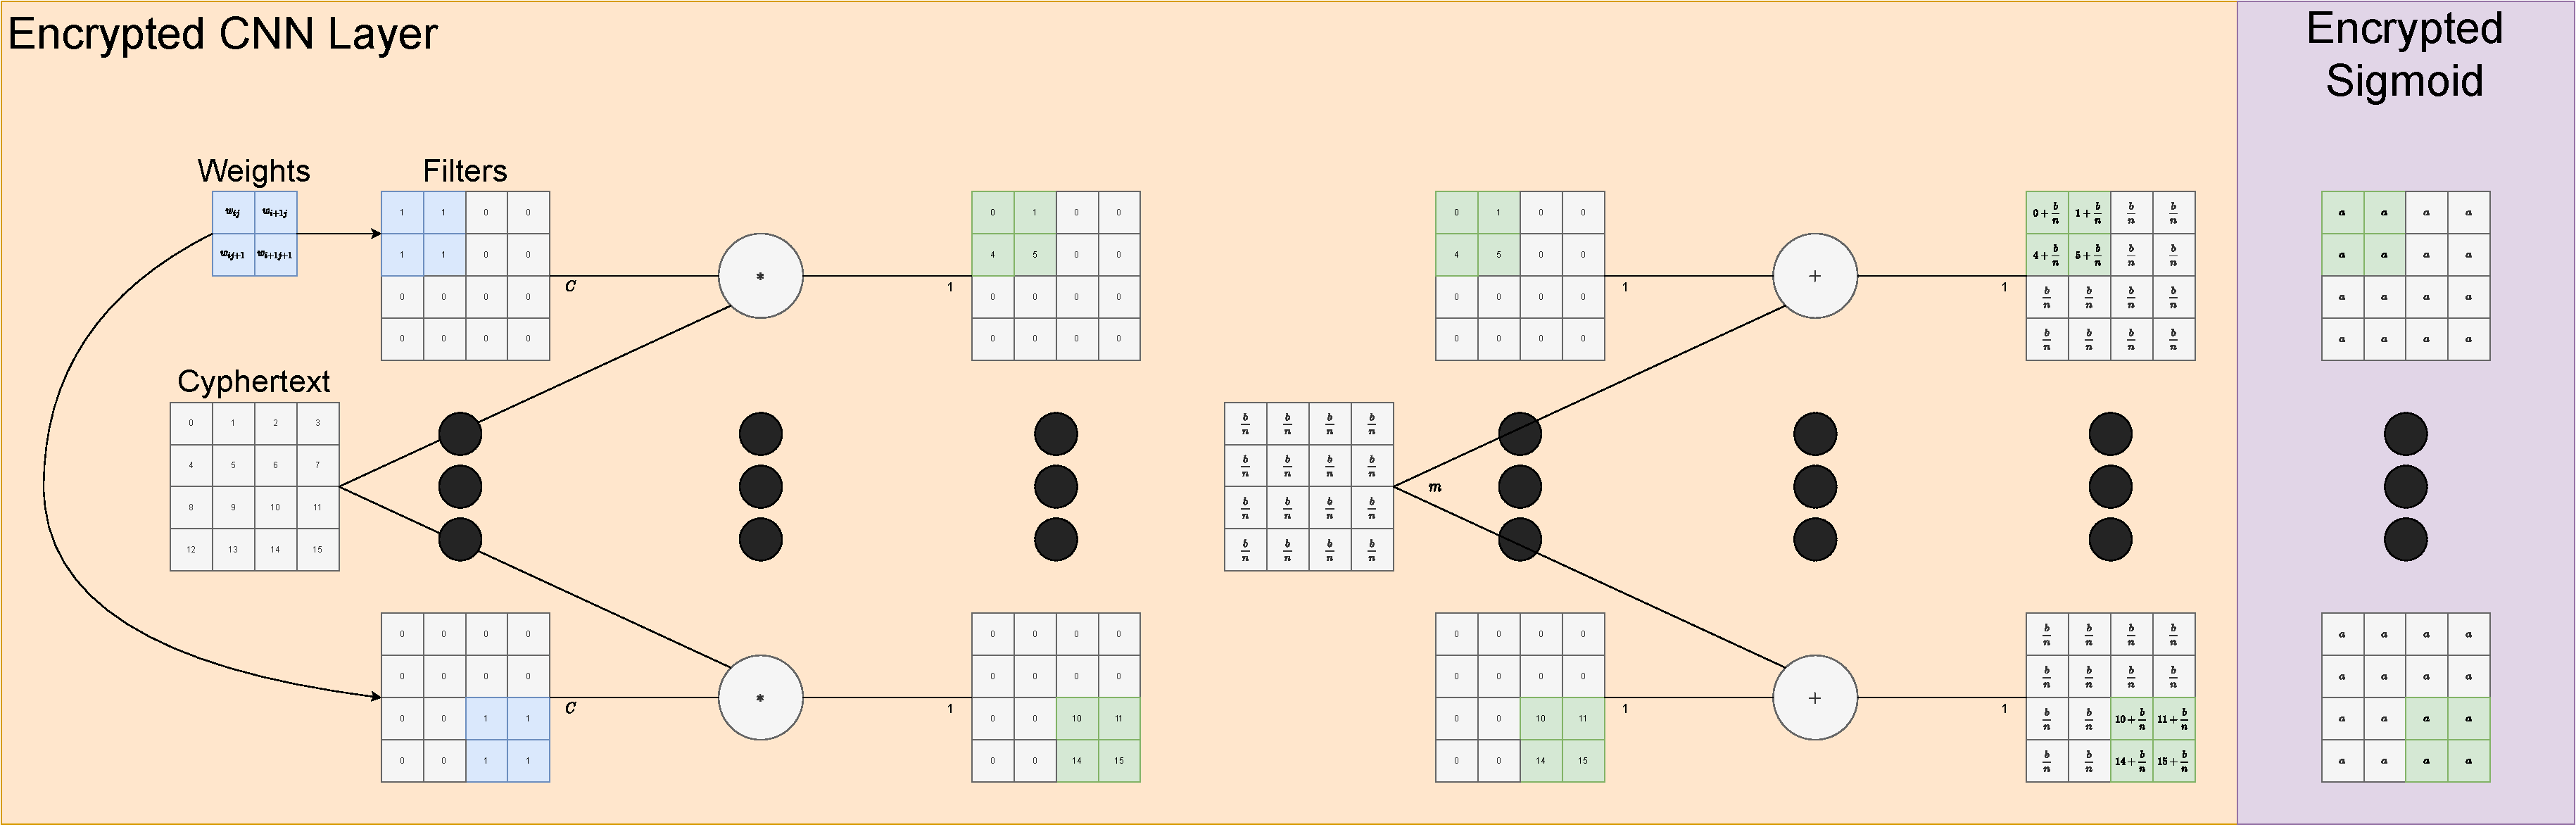
\includegraphics[width=0.7\textwidth]{cnn_computational_graph.pdf}
          \caption{FHE compatible convolutional neural network. \autocite{repository}}
          \label{fig:cnn_cg}
        \end{figure}
        \begin{figure}[th!]
          \centering
          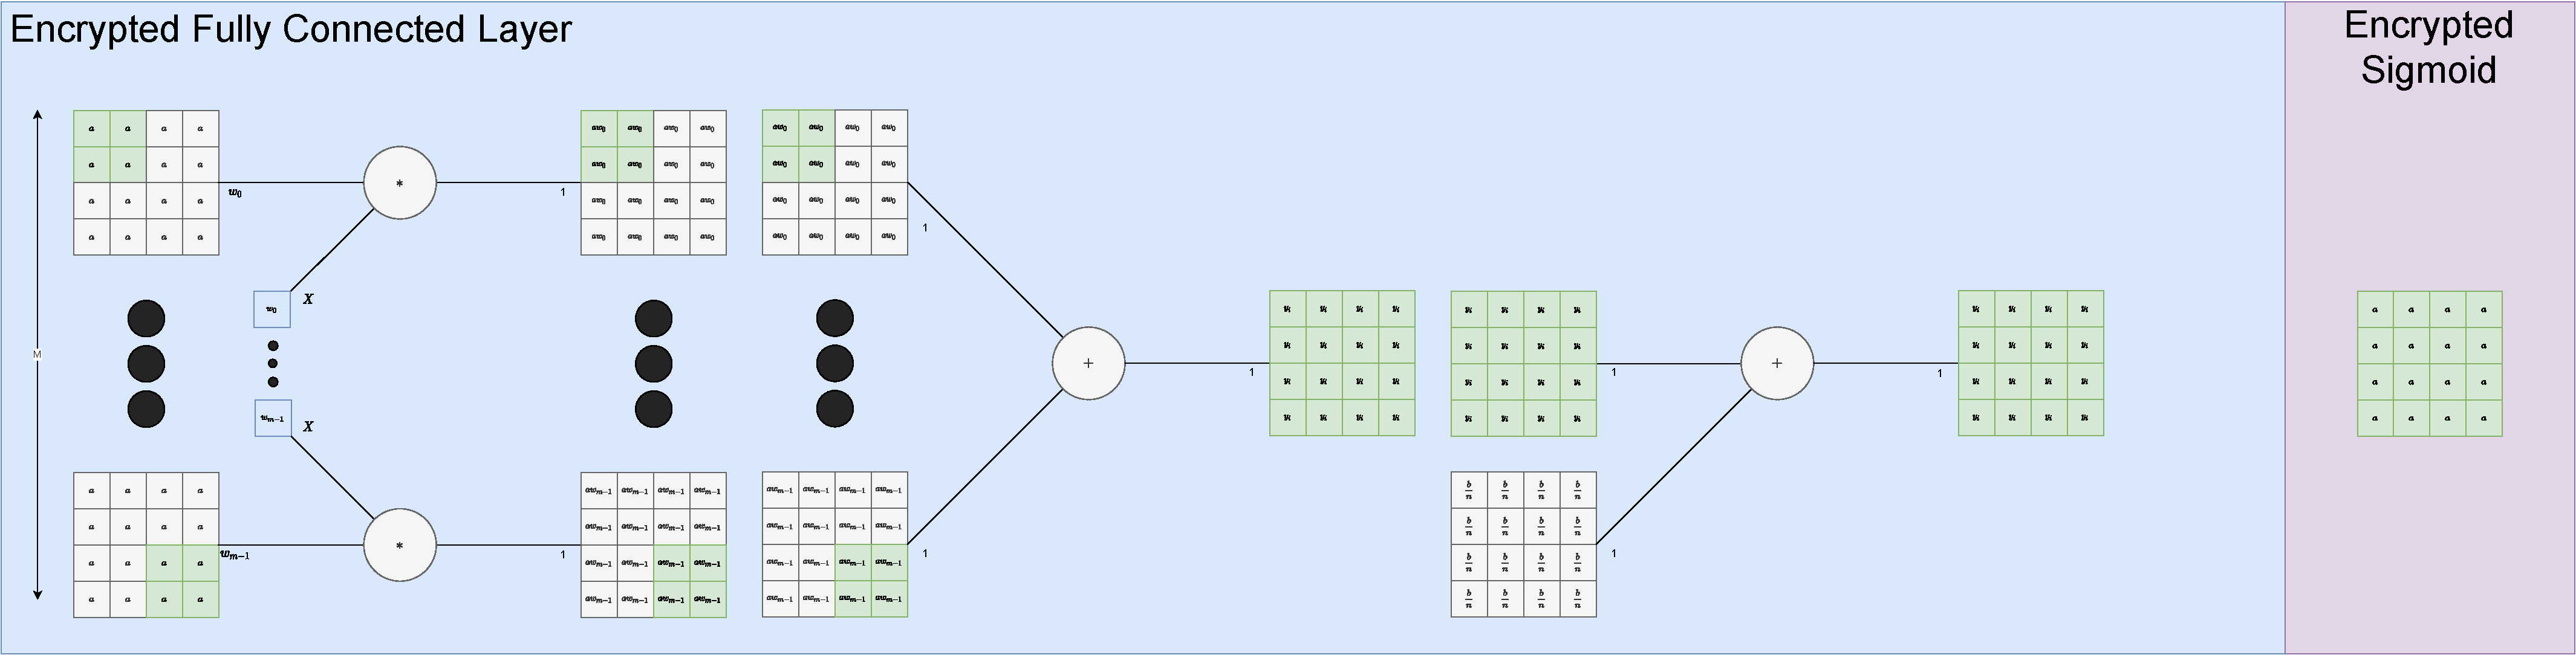
\includegraphics[width=0.7\textwidth]{dense_computational_graph.pdf}
          \caption{FHE compatible ANN/ Dense neural network. \autocite{repository}}
          \label{fig:ann_cg}
        \end{figure}
      \end{column}
    \end{columns}
  \end{frame}

% ----- FUTURE WORK PAGE
  \begin{frame}
    \frametitle{Future Work}
    \begin{columns}
      \begin{column}{0.5\textwidth}
        Starting to wrap everything up:
        \begin{itemize}
          \item Certainty metrics need implementing: Ensemble neural networks / Bayesian inference
          \item More papers are on their way/ imminent; Describe work thus far in greater detail
          \item Thesis!
        \end{itemize}
      \end{column}
      \begin{column}{0.5\textwidth}
        \begin{figure}[th!]
          \centering
          
\includegraphics[width=0.22\textwidth]{hal9000.pdf}
          \caption{Hal 9000, a space odyssey.}
          \label{fig:hal}
        \end{figure}
      \end{column}
    \end{columns}
  \end{frame}

% ----- REFERENCES PAGE
  \begin{frame}[allowframebreaks]
    \frametitle{References}
    % % biblatex version
    \printbibliography
  \end{frame}

% ----- QUESTIONS PAGE
  \begin{frame}
    \frametitle{Questions}
    \begin{columns}
      \begin{column}{0.5\textwidth}
        last chance to save link/ QR-code:
        \begin{itemize}
          \item https://github.com/DreamingRaven/ctp-presentations
          \item feel free to ask questions here if seeing this after the fact
        \end{itemize}
      \end{column}
      \begin{column}{0.5\textwidth}
        \begin{figure}[th!]
          \centering
          
\includegraphics[width=0.5\textwidth]{qrcode.png}
          \caption{QR code to this presentation for questions, and to my GitHub for projects. \autocite{repository}}
          \label{fig:qr}
        \end{figure}
      \end{column}
    \end{columns}
  \end{frame}


% ----- REFERENCES PAGE
  \begin{frame}
    \frametitle{Thanks}
    \begin{columns}
      \begin{column}{0.5\textwidth}
        Thanks to all of my supervisors:
        \begin{itemize}
          \item Georgios Leontidis
          \item Marc Hanheide
          \item Mark Else
          \item Richard Harnden
        \end{itemize}
      \end{column}
      \begin{column}{0.5\textwidth}
        Also thanks to the following:
        \begin{itemize}
          \item University of Lincoln (UoL)
          \item Berry Gardens Growers (BGG)
          \item National Institute of Agricultural Botany, East Malling Research (NIAB EMR)
          \item Biotechnology and Biological Sciences Research Council (BBSRC)
        \end{itemize}
      \end{column}
    \end{columns}
  \end{frame}


\end{document}
